\documentclass{article}
\usepackage{graphicx} % Required for inserting images
\usepackage{amsmath}
\usepackage[colorlinks=true, pdfstartview=FitV, linkcolor=blue, citecolor=blue, urlcolor=blue]{hyperref}
\usepackage{babel}
\usepackage{har2nat}
\usepackage{float}
\usepackage[top=1.1in, bottom=1.1in, left=1.15in, right=1.15in]{geometry}
\usepackage{booktabs}




\title{Lista 1 - Organização Industrial}
\author{Arthur M. Rodrigues}
\date{September 2023}

\begin{document}

\maketitle

\section*{Questão 1}

Como estamos interessados no impacto das características do carro sobre a demanda dos consumidores, imputar quantidade vendida igual para cada sub-modelo introduz um erro de medida na variável dependente que gera viés nas estimativas caso este erro esteja correlacionado com o vetor de características (i.e., caso a preferência dos consumidores por sub-modelos varie com as características). Por exemplo, se os consumidores demandam mais sub-modelos mais baratos do que submodelos mais caros, espera-se que parte do efeito do preço sobre demanda seja neutralizado ao analisar a base desagregada com quantidades iguais imputadas para todos os submodelos. Essa previsão é testável e será avaliada na Questão 4.

A alternativa proposta neste trabalho é agregar os dados de sub-modelo de forma a construir características representativas dos sub-modelos para cada um dos modelos da amostra. Para tal, consideramos a mediana das cilindradas, a média do preço e do IPI e construímos \emph{dummys} indicando se aquele modelo possui ao menos um sub-modelo com determinado tipo de combustível (álcool, gasolina, flex e diesel). Além disso, extraímos as características de número de portas, câmbio, válvulas e cavalos das descrições textuais dos sub-modelos, que foram agregadas a partir da média, moda, média e média, respectivamente. Entretanto, há uma quantidade grande de \emph{NAs} nessas características, de modo que elas não foram incluídas em algumas das especificações.

\section*{Questão 2}

Ao avaliar somente os 50 carros mais vendidos, não estamos lidando com o mercado completo, e sim com uma amostra provavelmente não representativa do mercado. Isso pode ser um problema, na medida em que, caso se incluísse os demais modelos na amostra, obteríamos, potencialmente, resultados econométricos diferentes.

Para tentar garantir a consistência das estimações, testaremos na Questão 4 uma especificação com uma subamostra contendo apenas os 35 modelos mais vendidos de cada ano: caso os resultados para a amostra com os 50 produtos mais vendidos sejam similares aos obtidos a partir da subamostra, teremos um indicativo de consistência. 

\section*{Questão 3}

Para modelar o \emph{outside good}, vamos utilizar dados do número de domicílios do Brasil, de acordo com a estratégia de \citeasnoun{berry1995automobile}. Estes dados foram obtidos através do Censo Demográfico de 2010, da Pesquisa Nacional por Amostra de Domicílios (PNAD) para 2003 a 2009 e da Pesquisa Nacional por Amostra de Domicílios Contínua Anual (PNADC/A) de 2016. Definimos a quantidade vendida do \emph{outside good} em determinado ano como o total de domicílios no Brasil naquele ano menos a soma da quantidade vendida de todos os modelos de carro contidos na base. Esta quantidade pode ser observada na Tabela \ref{tab out}:

\begin{table}[H]
    \centering
\begin{tabular}{r|r|r|r}
Ano & Domicílios (mil) & Outside Good (mil) & Market Share (\%)\\
\hline\hline
2003 & 50142 & 49315 & 0.983\\
\hline
2004 & 52158 & 51299 & 0.983\\
\hline
2005 & 53417 & 52550 & 0.983\\
\hline
2006 & 54817 & 53776 & 0.981\\
\hline
2007 & 56448 & 55089 & 0.975\\
\hline
2008 & 58282 & 56720 & 0.973\\
\hline
2009 & 59322 & 57467 & 0.968\\
\hline
2010 & 57428 & 55244 & 0.961\\
\hline
2011 & 62248 & 60124 & 0.965\\
\hline
2012 & 63854 & 61655 & 0.965\\
\hline
2013 & 65258 & 63002 & 0.965\\
\hline
2014 & 67131 & 65065 & 0.969\\
\hline
2015 & 68177 & 66612 & 0.977\\
\hline
2016 & 67213 & 65996 & 0.981\\
\hline
\end{tabular}
    \caption{"Vendas" do \emph{outside good} por ano (2003 - 2016)}
    \label{tab out}
\end{table}

Como podemos verificar, a imensa maioria dos domicílios não compra um carro novo em um dado ano. Este indicador tem leve tendência de queda durante a série histórica e volta a subir no final do período analisado com a crise econômica de 2015-2016.

\section*{Questão 4}\label{sec4}

Considere indivíduos indexados por $i \in \{1, ..., I\}$ e bens indexados por $j \in \{0, 1, ..., J\}$ produzidos por firmas indexadas por $f \in \{1, ..., F\}$, em que a utilidade do indivíduo $i$ ao comprar o bem $j$ é dada por:

\begin{equation}
    u_{ij} = \delta_j + \epsilon_{ij}
\end{equation}

Em que, de modo geral, $\delta_j = X_j \cdot \beta$ e $\epsilon_{ij} \sim Gumbel(0)$. Note que $X_j$ é um vetor arbitrário de características do carro, das quais convém destacar o preço, com $\delta_j = \alpha p_j + X_j \cdot \beta$; ou em alguns casos adicionar efeitos fixos de ano e de marca, de acordo com a especificação de \citeasnoun{nevo2001measuring}, com $\delta_{jt} = \alpha p_{jt} + \beta \cdot X_{jt} + \theta_t + \nu_k$. Pelas propriedades da distribuição Gumbel, temos que:

\begin{equation}
    P( j \: \text{escolhido}) = P (u_{ij} > u_{ik} \forall k \neq j) = \frac{e^{\delta_j}}{\sum_{k = 0}^J e^{\delta_k}}
\end{equation}

Vamos tomar o \emph{outside good} como um bem com todas as características iguais a 0, de modo que $P( j \: \text{escolhido}) = \frac{e^{\delta_j}}{1 + \sum_{k = 1}^J e^{\delta_k}}$. Defina o market share de $j$ como $s_j = \frac{\text{vendas de}\:j}{\text{pop. total}} \approx P(j \: \text{escolhido})$. Dividindo o market share do bem $j$ pelo outside good, temos $\frac{s_j}{s_0} = \frac{e^{\delta_j}}{e^{\delta_0}} = e^{\delta_j}$. Substituindo $\delta_j$ pelas características da base, vamos estimar o modelo a partir da equação

\begin{equation}
    log(s_{jt}) - log(s_{0t}) = \alpha p_{jt} + \theta_t + \nu_k + \beta \cdot X_{jt} + xi_{jt} 
\end{equation}

Onde $\theta_t$ representa um efeito fixo de tempo, $\nu_k$ representa um efeito fixo de marca e $X_{jt}$ é um vetor de características que contém cilindradas, tipo de combustível (com a gasolina omitida em função da multicolinearidade), número de portas, válvulas, cavalos e tipo de câmbio. $\xi_{jt}$ é um termo de erro. Algumas características ou efeitos fixos foram omitidos de algumas das regressões, e um resumo dos resultados pode ser observado na Tabela \ref{tablogit}:
\begin{table}[H]

\begingroup
\centering
\begin{tabular}{lcccc}
   \tabularnewline \midrule \midrule
   Dependent Variable: & \multicolumn{4}{c}{y}\\
   Model:        & (1)                           & (2)                           & (3)                            & (4)\\  
   \midrule
   \emph{Variables}\\
   preco\_media  & $-2.5\times 10^{-5}$$^{***}$  & $-2.4\times 10^{-5}$$^{***}$  & $-1.82\times 10^{-5}$$^{***}$  & $-1.39\times 10^{-5}$$^{**}$\\    
                 & ($4.5\times 10^{-6}$)         & ($4\times 10^{-6}$)           & ($2.03\times 10^{-6}$)         & ($5.84\times 10^{-6}$)\\    
   cc\_mediana   & -0.3370                       & -0.3359                       & 0.1134                         & -0.4994\\   
                 & (0.2335)                      & (0.2517)                      & (0.0912)                       & (0.3030)\\   
   alcool        & 0.4878$^{**}$                 & -0.0248                       &                                &   \\   
                 & (0.2004)                      & (0.1628)                      &                                &   \\   
   diesel        & 0.3347                        & 0.0002                        & 0.2599                         & -0.0906\\   
                 & (0.2785)                      & (0.3334)                      & (0.1783)                       & (0.1080)\\   
   flex          & 0.5818$^{***}$                & 0.8827$^{***}$                & 0.4582$^{***}$                 & 0.5167$^{**}$\\   
                 & (0.1171)                      & (0.2793)                      & (0.0899)                       & (0.2383)\\   
   cambioMec     &                               &                               & 0.3722$^{***}$                 & 0.1624\\   
                 &                               &                               & (0.1160)                       & (0.1442)\\   
   valvulas      &                               &                               &                                & 0.0508\\   
                 &                               &                               &                                & (0.0532)\\   
   portas        &                               &                               &                                & 0.1512\\   
                 &                               &                               &                                & (0.1848)\\   
   \midrule
   \emph{Fixed-effects}\\
   ano\_ref      & Yes                           &                               & Yes                            & Yes\\  
   marca         & Yes                           & Yes                           & Yes                            & Yes\\  
   \midrule
   \emph{Fit statistics}\\
   Observations  & 498                           & 498                           & 183                            & 111\\  
   R$^2$         & 0.60788                       & 0.53844                       & 0.69421                        & 0.70234\\  
   Within R$^2$  & 0.45846                       & 0.44081                       & 0.35323                        & 0.25323\\  
   \midrule \midrule
   \multicolumn{5}{l}{\emph{Signif. Codes: ***: 0.01, **: 0.05, *: 0.1}}\\
\end{tabular}
\par\endgroup
\caption{Resultados Logit - Base Completa Agregada}\label{tablogit}
\end{table}

O coeficiente de preços possui o sentido esperado e é relativamente estável e estatisticamente significante nas quatro especificações (na última delas, apenas a 5\%). Parece haver uma predileção por carros com combustível de álcool\footnote{O coeficiente de álcool não pode ser calculado nas especificações 3 e 4 porque não há nenhum carro movido a álcool com câmbio automático na amostra.} ou flex, possivelmente explicados pelo menor consumo de combustível.


Este modelo logit simples nos permite avaliar os dois questionamentos levantados nas Questões 1 e 2. Em primeiro lugar, vamos rodar o mesmo modelo com a base restrita para avaliarr se os coeficientes de preço se mantêm estáveis. Os resultados podem ser observados na Tabela \ref{tablogitrest}.

\begin{table}[H]
\begingroup
\centering
\begin{tabular}{lcccc}
   \tabularnewline \midrule \midrule
   Dependent Variable: & \multicolumn{4}{c}{y}\\
   Model:        & (1)                            & (2)                            & (3)                           & (4)\\  
   \midrule
   \emph{Variables}\\
   preco\_media  & $-2.46\times 10^{-5}$$^{***}$  & $-2.38\times 10^{-5}$$^{***}$  & $-1.8\times 10^{-5}$$^{***}$  & $-1.21\times 10^{-5}$$^{*}$\\    
                 & ($4.61\times 10^{-6}$)         & ($3.56\times 10^{-6}$)         & ($3.97\times 10^{-6}$)        & ($6.53\times 10^{-6}$)\\    
   cc\_mediana   & -0.4326$^{*}$                  & -0.4681                        & 0.0732                        & -0.6174\\   
                 & (0.2407)                       & (0.2861)                       & (0.1450)                      & (0.3501)\\   
   alcool        & 0.4597$^{**}$                  & -0.0478                        &                               &   \\   
                 & (0.2022)                       & (0.1399)                       &                               &   \\   
   diesel        & -0.4934$^{**}$                 & -0.7177$^{*}$                  & -0.0517                       & -0.1145\\   
                 & (0.2198)                       & (0.3703)                       & (0.1307)                      & (0.1275)\\   
   flex          & 0.6000$^{***}$                 & 0.9447$^{***}$                 & 0.4370$^{***}$                & 0.5059$^{*}$\\   
                 & (0.1036)                       & (0.2979)                       & (0.1089)                      & (0.2628)\\   
   cambioMec     &                                &                                & 0.3579$^{**}$                 & 0.1441\\   
                 &                                &                                & (0.1301)                      & (0.1607)\\   
   valvulas      &                                &                                &                               & 0.0530\\   
                 &                                &                                &                               & (0.0536)\\   
   portas        &                                &                                &                               & 0.1704\\   
                 &                                &                                &                               & (0.1911)\\   
   \midrule
   \emph{Fixed-effects}\\
   ano\_ref      & Yes                            &                                & Yes                           & Yes\\  
   marca         & Yes                            & Yes                            & Yes                           & Yes\\  
   \midrule
   \emph{Fit statistics}\\
   Observations  & 468                            & 468                            & 168                           & 106\\  
   R$^2$         & 0.62517                        & 0.55383                        & 0.68570                       & 0.69096\\  
   Within R$^2$  & 0.45276                        & 0.45720                        & 0.31356                       & 0.25411\\  
   \midrule \midrule
   \multicolumn{5}{l}{\emph{Signif. Codes: ***: 0.01, **: 0.05, *: 0.1}}\\
\end{tabular}
\par\endgroup
    \caption{Resultados Logit - Base Restrita Agregada}
    \label{tablogitrest}
\end{table}

É possível observar que o sentido e magnitude dos coeficiente de preço no modelo restrito se mantêm consistentes na amostra restrita. O último coeficiente de preço é significativo apenas a 10\%, mas isto pode ser explicado pelo erro padrão maior decorrente da amostra reduzida. De modo geral, os resultados da estimação na amostra reduzida estão em consonância com a tese de que a amostra de 50 veículos mais vendidos é uma aproximação razoável para o mercado. Além disso, realizamos o mesmo exercício com a base desagregada, com os resultados na Tabela \ref{tablogitdes}.


\begin{table}[H]

\begingroup
\centering
\begin{tabular}{lcccc}
   \tabularnewline \midrule \midrule
   Dependent Variable: & \multicolumn{4}{c}{y}\\
   Model:       & (1)                            & (2)                     & (3)                     & (4)\\  
   \midrule
   \emph{Variables}\\
   preco        & $-1.02\times 10^{-5}$$^{***}$  & $-7.92\times 10^{-6}$   & $-1.1\times 10^{-6}$    & $6.24\times 10^{-6}$$^{**}$\\    
                & ($1.46\times 10^{-6}$)         & ($5.11\times 10^{-6}$)  & ($1.19\times 10^{-6}$)  & ($2.59\times 10^{-6}$)\\    
   cc           & -0.3620$^{***}$                & -0.3847$^{*}$           & -0.0751                 & -0.4822$^{**}$\\   
                & (0.0562)                       & (0.2115)                & (0.0987)                & (0.1994)\\   
   alcool       & 0.1954                         & 0.0139                  &                         &   \\   
                & (0.1166)                       & (0.3241)                &                         &   \\   
   diesel       & 0.1188                         & 0.3023$^{**}$           & -0.0738                 &   \\   
                & (0.0866)                       & (0.1222)                & (0.0610)                &   \\   
   flex         & -0.0300                        & 0.3182$^{**}$           & 0.0812                  & 0.1085\\   
                & (0.0434)                       & (0.1482)                & (0.0638)                & (0.0995)\\   
   cambioMec    &                                &                         & 0.0655                  & 0.1172$^{**}$\\   
                &                                &                         & (0.0423)                & (0.0411)\\   
   valvulas     &                                &                         &                         & 0.0125\\   
                &                                &                         &                         & (0.0095)\\   
   portas       &                                &                         &                         & 0.1302$^{***}$\\   
                &                                &                         &                         & (0.0312)\\   
   \midrule
   \emph{Fixed-effects}\\
   ano\_ref     & Yes                            &                         & Yes                     & Yes\\  
   marca        & Yes                            & Yes                     & Yes                     & Yes\\  
   \midrule
   \emph{Fit statistics}\\
   Observations & 4,351                          & 4,351                   & 1,629                   & 789\\  
   R$^2$        & 0.45242                        & 0.36815                 & 0.61631                 & 0.52148\\  
   Within R$^2$ & 0.13248                        & 0.12864                 & 0.01533                 & 0.03332\\  
   \midrule \midrule
   \multicolumn{5}{l}{\emph{Signif. Codes: ***: 0.01, **: 0.05, *: 0.1}}\\
\end{tabular}
\par\endgroup
\caption{Resultados Logit - Base Completa Desagregada}\label{tablogitdes}
\end{table}

Neste exercício, o coeficiente de preço não é estatisticamente significante na terceira regressão e é estatisticamente significante com sinal positivo (contrário ao esperado pela teoria econômica) na quarta especificação. Assim, parece haver fundamento na tese de que há predileção por preço dentro dos submodelos e de que trabalhar com a base desagregada não é o ideal. Portanto, a partir da questão 5 realizaremos todos os exercícios de estimação exclusivamente na base agregada e completa.

\section*{Questão 5}

Para lidar com a endogeneidade no preço, vamos utilizar o IPI como instrumento. Para tal, necessitamos que ele satisfaça as condições de restrição e exclusão. A alíquota do IPI é calculada a partir de uma série de fatores, dentre eles as cilindradas do carro e o tipo de combustível, além de incidir no momento da venda, de forma a impactar diretamente no preço. Por impactar positivamente no preço, reduziria a quantidade comprada. A relevância do IPI sobre a quantidade se reflete a partir de sua composição no preço, portanto,  no primeiro estágio, em que o preço é regredido no IPI e nas demais variáveis. Espera-se, assim, que o IPI exerça um efeito positivo sobre o preço.

A condição de exclusão, todavia, não é testável. De qualquer forma, pode-se argumentar que a única forma que o IPI afeta a quantidade de vendas de certo modelo é por meio de seu efeito no preço, uma vez que sua incidência é direta no preço. Por outro lado, o IPI poderia ferir a condição de exogeneidade caso alguma parte da composição do IPI estivesse ligada a uma variável não observável que afeta a demanda, como tamanho do carro. Os resultados da forma reduzida da regressão por IV podem ser encontrados na Tabela \ref{tab:iv}:

\begin{table}[H]
\begingroup
\centering
\begin{tabular}{lcccc}
   \tabularnewline \midrule \midrule
   Dependent Variable: & \multicolumn{4}{c}{y}\\
   Model:        & (1)                     & (2)                            & (3)                     & (4)\\  
   \midrule
   \emph{Variables}\\
   preco\_media  & -0.0001$^{***}$         & $-5.42\times 10^{-5}$$^{***}$  & $-2.17\times 10^{-5}$   & -0.0002\\   
                 & ($4.69\times 10^{-5}$)  & ($1.41\times 10^{-5}$)         & ($1.55\times 10^{-5}$)  & (0.0003)\\   
   alcool        & -0.3891                 & 0.3358                         &                         &   \\   
                 & (0.4978)                & (0.2508)                       &                         &   \\   
   diesel        & -0.0846                 & 2.006$^{***}$                  & 0.2694                  & 0.6079\\   
                 & (0.6552)                & (0.4392)                       & (0.3139)                & (1.434)\\   
   flex          & 0.3697$^{*}$            & 0.4249$^{***}$                 & 0.4570$^{***}$          & 1.565\\   
                 & (0.2106)                & (0.1323)                       & (0.1224)                & (1.615)\\   
   cc\_mediana   & 3.390$^{**}$            & 0.9463$^{*}$                   & 0.2526                  & 4.092\\   
                 & (1.694)                 & (0.5570)                       & (0.6288)                & (6.573)\\   
   cambioMec     &                         &                                & 0.3545$^{***}$          & -0.4879\\   
                 &                         &                                & (0.1225)                & (0.9982)\\   
   portas        &                         &                                &                         & 0.1698\\   
                 &                         &                                &                         & (0.3705)\\   
   valvulas      &                         &                                &                         & 0.4102\\   
                 &                         &                                &                         & (0.5199)\\   
   \midrule
   \emph{Fixed-effects}\\
   ano\_ref      & Yes                     & Yes                            & Yes                     & Yes\\  
   marca         & Yes                     &                                & Yes                     & Yes\\  
   \midrule
   \emph{Fit statistics}\\
   Observations  & 498                     & 498                            & 183                     & 111\\  
   R$^2$         & -0.29387                & 0.31396                        & 0.69274                 & -0.95555\\  
   Within R$^2$  & -0.78687                & 0.22213                        & 0.35012                 & -3.9061\\  
   \midrule \midrule
   \multicolumn{5}{l}{\emph{IID standard-errors in parentheses}}\\
   \multicolumn{5}{l}{\emph{Signif. Codes: ***: 0.01, **: 0.05, *: 0.1}}\\
\end{tabular}
\par\endgroup
    \caption{Regressão IV}
    \label{tab:iv}
\end{table}


Percebe-se que nesta especificação, o preço exerce um efeito negativo sobre a quantidade vendida - trivialmente - porém com magnitude maior (em módulo) do que no Logit realizado na Questão 4. Ao lidar com a endogeneidade, encontramos a demanda consideravelmente mais sensível ao preço, o que indica que havia viés nos coeficientes estimados por OLS. Os resultados da regressão de 1º Estágio podem ser observados na Tabela \ref{tab:1es}.

\begin{table}[H]
\begingroup
\centering
\begin{tabular}{lcccc}
   \tabularnewline \midrule \midrule
   Dependent Variable: & \multicolumn{4}{c}{preco\_media}\\
   Model:       & (1)               & (2)               & (3)               & (4)\\  
   \midrule
   \emph{Variables}\\
   ipi          & 139,561.0$^{***}$ & 283,427.3$^{***}$ & 360,433.0$^{***}$ & 139,561.0$^{***}$\\   
                & (52,309.9)        & (50,865.7)        & (103,639.5)       & (52,309.9)\\   
   alcool       & -8,498.6$^{***}$  & -9,835.4$^{***}$  &                   & -8,498.6$^{***}$\\   
                & (2,405.3)         & (2,633.9)         &                   & (2,405.3)\\   
   diesel       & -2,677.5          & 28,406.7$^{***}$  & 7,325.3           & -2,677.5\\   
                & (5,042.2)         & (3,603.8)         & (5,910.8)         & (5,042.2)\\   
   flex         & -984.4            & -1,865.8          & 3,239.8           & -984.4\\   
                & (1,551.4)         & (1,562.0)         & (2,481.9)         & (1,551.4)\\   
   cc\_mediana  & 32,118.9$^{***}$  & 31,204.8$^{***}$  & 28,439.4$^{***}$  & 32,118.9$^{***}$\\   
                & (1,928.6)         & (1,891.7)         & (4,484.4)         & (1,928.6)\\   
   cambioMec    &                   &                   & -5,767.0$^{***}$  &   \\   
                &                   &                   & (1,788.5)         &   \\   
   \midrule
   \emph{Fixed-effects}\\
   ano\_ref     & Yes               & Yes               & Yes               & Yes\\  
   marca        & Yes               &                   & Yes               & Yes\\  
   \midrule
   \emph{Fit statistics}\\
   Observations & 498               & 498               & 183               & 498\\  
   R$^2$        & 0.83360           & 0.77753           & 0.87670           & 0.83360\\  
   Within R$^2$ & 0.66331           & 0.76523           & 0.57065           & 0.66331\\  
   \midrule \midrule
   \multicolumn{5}{l}{\emph{IID standard-errors in parentheses}}\\
   \multicolumn{5}{l}{\emph{Signif. Codes: ***: 0.01, **: 0.05, *: 0.1}}\\
\end{tabular}
\par\endgroup
    \caption{Primeiro Estágio}
    \label{tab:1es}
\end{table}

Percebe-se, a partir da regressão de primeiro estágio, que a condição de relevância é atendida, na medida em que o IPI apresenta um efeito positivo e significativo a 1\% sobre o preço para todas as especificações.

\section*{Questão 6}
Para calcular as elasticidades, vamos utilizar a formula derivada na Questão 4, de $s_j = \frac{e^{\delta_j}}{\sum_{k = 0}^J e^{\delta_k}}$, com $\delta_j = \alpha p_j + \beta \cdot X_j$. Portanto, a elasticidade da demanda do bem $j$ pelo bem $k$ é:

$$
e_{j,k} = \frac{\partial s_j}{\partial p_k} \frac{p_k}{s_j} = \begin{cases}-\alpha p_{j}\left(1-s_{j}\right) & \text { se } j=k \\ \alpha p_{k} s_{k} & \text { c.c. }\end{cases}
$$

Para computarmos a elasticidade-preço da demanda do Gol, utilizaremos o valor de $\hat{\alpha}$ estimado na especificação (1) da regressão de IV, isto é, com efeitos fixos de ano e marca com as características de combustível, cilindradas e preço, que estão presentes em todos os carros da amostra. Os resultados para o ano de 2016 (o mais recente da amostra) podem ser observados na Tabela \ref{tab:elastlogit}.

\begin{table}[H]
\centering
\begin{tabular}{l|l|r|r|r}
Marca & Modelo & Quantidade & Market Share & Elasticidade\\
\hline\hline
PEUGEOT & 2008 & 10692 & 0.0001591 & 0.0015220\\
\hline
PEUGEOT & 208 & 10768 & 0.0001602 & 0.0011666\\
\hline
CITROEN & C3 & 11824 & 0.0001759 & 0.0012246\\
\hline
HONDA & CITY & 15422 & 0.0002294 & 0.0020223\\
\hline
HONDA & CIVIC & 20857 & 0.0003103 & 0.0035805\\
\hline
GM & CLASSIC & 11530 & 0.0001715 & 0.0007351\\
\hline
RENAULT & CLIO & 10869 & 0.0001617 & 0.0006177\\
\hline
GM & COBALT & 22466 & 0.0003343 & 0.0023814\\
\hline
JEEP & COMPASS & 6599 & 0.0000982 & 0.0013690\\
\hline
TOYOTA & COROLLA & 64740 & 0.0009632 & 0.0102810\\
\hline
RENAULT & DUSTER & 25373 & 0.0003775 & 0.0033982\\
\hline
FORD & ECOSPORT & 28105 & 0.0004181 & 0.0039380\\
\hline
HONDA & FIT & 28439 & 0.0004231 & 0.0034717\\
\hline
FORD & FOCUS & 6766 & 0.0001007 & 0.0010477\\
\hline
VW & GOL & 57390 & 0.0008539 & -5.4308072\\
\hline
HYUNDAI & HB20 & 121616 & 0.0018094 & 0.0116433\\
\hline
HYUNDAI & HB20S & 46023 & 0.0006847 & 0.0048706\\
\hline
HONDA & HR-V & 55758 & 0.0008296 & 0.0093391\\
\hline
HYUNDAI & IX35 & 10226 & 0.0001521 & 0.0022160\\
\hline
VW & JETTA & 8654 & 0.0001288 & 0.0013839\\
\hline
RENAULT & LOGAN & 23707 & 0.0003527 & 0.0022138\\
\hline
NISSAN & MARCH & 18376 & 0.0002734 & 0.0015775\\
\hline
FIAT & MOBI & 28731 & 0.0004275 & 0.0021451\\
\hline
GM & ONIX & 153371 & 0.0022819 & 0.0137919\\
\hline
FIAT & PALIO & 63996 & 0.0009521 & 0.0062821\\
\hline
GM & PRISMA & 66337 & 0.0009870 & 0.0065397\\
\hline
FIAT & PUNTO & 7709 & 0.0001147 & 0.0008522\\
\hline
JEEP & RENEGADE & 51563 & 0.0007672 & 0.0098042\\
\hline
RENAULT & SANDERO & 63228 & 0.0009407 & 0.0061233\\
\hline
NISSAN & SENTRA & 6288 & 0.0000936 & 0.0010009\\
\hline
FIAT & SIENA & 33478 & 0.0004981 & 0.0024763\\
\hline
GM & SPIN & 22982 & 0.0003419 & 0.0026922\\
\hline
GM & TRACKER & 8558 & 0.0001273 & 0.0013071\\
\hline
HYUNDAI & TUCSON & 11203 & 0.0001667 & 0.0014995\\
\hline
FIAT & UNO & 34626 & 0.0005152 & 0.0026811\\
\hline
NISSAN & VERSA & 21897 & 0.0003258 & 0.0022733\\
\hline
VW & VOYAGE & 26074 & 0.0003879 & 0.0024990\\
\hline
\end{tabular}
    \caption{Elasticidades Logit IV - 2016}
    \label{tab:elastlogit}
\end{table}

Conforme esperado, o único modelo com elasticidade cruzada negativa com o Gol é ele mesmo. Além disso, existe uma relação aproximadamente linear entre a quantidade vendida e a elasticidade cruzada com o Gol, conforme pode ser visto na Figura \ref{fig:elastlogit}. Esta relação é esperada, visto que a fórmula da elasticidade derivada acima depende diretamente e linearmente do nível de preços.

\begin{figure}[H]
    \centering
    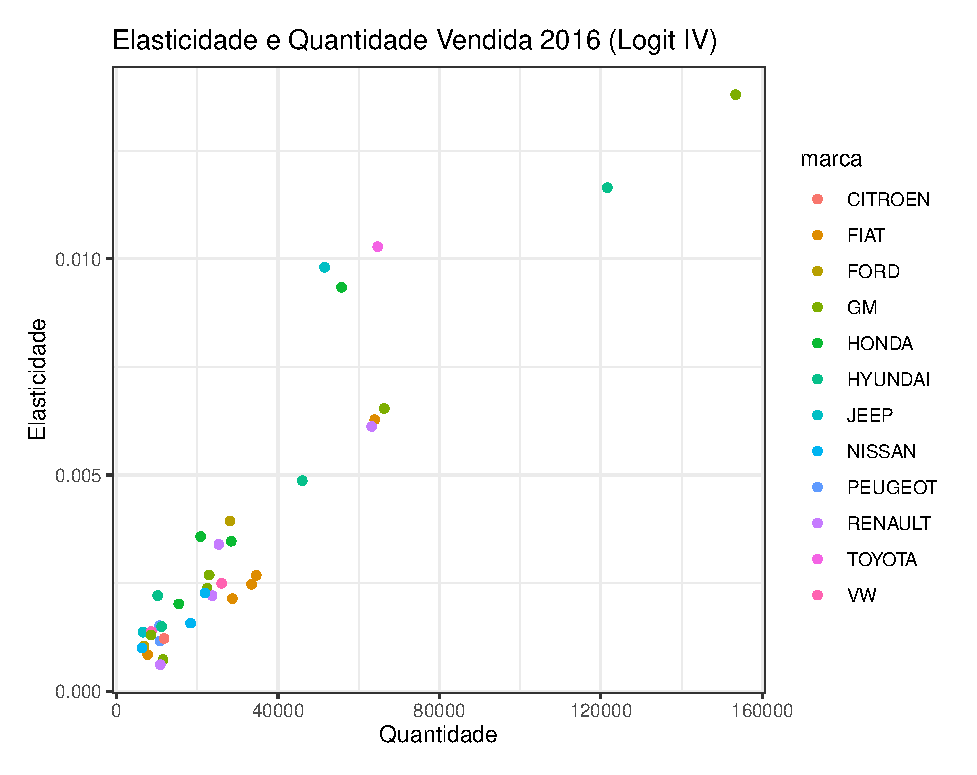
\includegraphics{figs and tabs/elasticidadesiv.eps}
    \caption{Elasticidade e Quantidade Vendida 2016 - Logit IV}
    \label{fig:elastlogit}
\end{figure}

\section*{Questão 7}

Para estimar os custos, vamos modelar a oferta de acordo com a formulação de \citeasnoun{berry1995automobile}. Considere firmas indexadas por $f \in \{1, ..., F\}$, em que cada produto $j$ é produzido por uma única firma $f$, e suponha conduta de competição oligopolística de Bertrand-Nash. Defina $c'_j$ como o custo marginal do bem $j$ e $M$ o número de domicílios do mercado. Assim, cada firma $f$ terá o problema:

$$
\max_{\{p_j\}_f} \Pi_f = \sum\limits_{j\text{ de }f} (p_j - c'_j) M s_j
$$

Deste problema, derivamos as CPOs:

$$
s_j - \sum_r (p_r - c'_r)\Delta_{jr} = 0
$$

Onde $\Delta_{jr} = \begin{cases}-\frac{\partial s_r}{\partial p_j} & \text { se } j=k \\ 0 & \text { c.c. }\end{cases}$. Assim, temos uma fórmula para o custo marginal em função da inversa da matriz $\Delta$:

$$
c' = p - \Delta^{-1}s
$$

Com este resultado, obtemos os markups a partir de:

$$markup =(p - c') / c'$$

Os resultados deste exercício no modelo de Logit para o ano de 2016 podem ser observados na Tabela \ref{tab:custologit}:

\begin{table}[H]
\centering
\begin{tabular}{l|l|r|r|r|r}
Marca & Modelo & Preço & Market Share & Custo Marginal & Markup\\
\hline\hline
PEUGEOT & 2008 & 74405.20 & 0.0001591 & 66626.28 & 0.1167545\\
\hline
PEUGEOT & 208 & 56625.92 & 0.0001602 & 48847.01 & 0.1592506\\
\hline
CITROEN & C3 & 54131.93 & 0.0001759 & 46354.13 & 0.1677909\\
\hline
HONDA & CITY & 68537.75 & 0.0002294 & 60747.35 & 0.1282426\\
\hline
HONDA & CIVIC & 89727.80 & 0.0003103 & 81937.40 & 0.0950774\\
\hline
GM & CLASSIC & 33323.00 & 0.0001715 & 25513.42 & 0.3060967\\
\hline
RENAULT & CLIO & 29702.67 & 0.0001617 & 21911.96 & 0.3555461\\
\hline
GM & COBALT & 55402.88 & 0.0003343 & 47593.30 & 0.1640898\\
\hline
JEEP & COMPASS & 108433.00 & 0.0000982 & 100649.83 & 0.0773292\\
\hline
TOYOTA & COROLLA & 83003.17 & 0.0009632 & 75219.24 & 0.1034832\\
\hline
RENAULT & DUSTER & 70001.62 & 0.0003775 & 62210.91 & 0.1252306\\
\hline
FORD & ECOSPORT & 73237.09 & 0.0004181 & 65456.62 & 0.1188645\\
\hline
HONDA & FIT & 63805.50 & 0.0004231 & 56015.10 & 0.1390767\\
\hline
FORD & FOCUS & 80937.12 & 0.0001007 & 73156.66 & 0.1063535\\
\hline
VW & GOL & 42268.40 & 0.0008539 & 34481.29 & 0.2258357\\
\hline
HYUNDAI & HB20 & 50040.38 & 0.0018094 & 42242.01 & 0.1846117\\
\hline
HYUNDAI & HB20S & 55314.75 & 0.0006847 & 47516.38 & 0.1641196\\
\hline
HONDA & HR-V & 87544.75 & 0.0008296 & 79754.35 & 0.0976799\\
\hline
HYUNDAI & IX35 & 113267.50 & 0.0001521 & 105469.13 & 0.0739398\\
\hline
VW & JETTA & 83585.14 & 0.0001288 & 75798.04 & 0.1027349\\
\hline
RENAULT & LOGAN & 48809.56 & 0.0003527 & 41018.84 & 0.1899300\\
\hline
NISSAN & MARCH & 44870.36 & 0.0002734 & 37088.53 & 0.2098175\\
\hline
FIAT & MOBI & 39023.00 & 0.0004275 & 31227.02 & 0.2496550\\
\hline
GM & ONIX & 47001.71 & 0.0022819 & 39192.14 & 0.1992638\\
\hline
FIAT & PALIO & 51307.85 & 0.0009521 & 43511.86 & 0.1791691\\
\hline
GM & PRISMA & 51526.86 & 0.0009870 & 43717.28 & 0.1786382\\
\hline
FIAT & PUNTO & 57782.55 & 0.0001147 & 49986.56 & 0.1559615\\
\hline
JEEP & RENEGADE & 99382.43 & 0.0007672 & 91599.26 & 0.0849698\\
\hline
RENAULT & SANDERO & 50618.43 & 0.0009407 & 42827.72 & 0.1819081\\
\hline
NISSAN & SENTRA & 83199.83 & 0.0000936 & 75418.01 & 0.1031826\\
\hline
FIAT & SIENA & 38661.00 & 0.0004981 & 30865.02 & 0.2525831\\
\hline
GM & SPIN & 61227.88 & 0.0003419 & 53418.30 & 0.1461966\\
\hline
GM & TRACKER & 79829.50 & 0.0001273 & 72019.92 & 0.1084363\\
\hline
HYUNDAI & TUCSON & 69960.00 & 0.0001667 & 62161.63 & 0.1254531\\
\hline
FIAT & UNO & 40471.44 & 0.0005152 & 32675.46 & 0.2385883\\
\hline
NISSAN & VERSA & 54264.00 & 0.0003258 & 46482.18 & 0.1674152\\
\hline
VW & VOYAGE & 50094.64 & 0.0003879 & 42307.53 & 0.1840596\\
\hline
\end{tabular}
    \caption{Custos Marginais e Markup Logit - 2016}
    \label{tab:custologit}
\end{table}

Os resultados apresentam markups e custos marginais relativamente dependentes dos preços e market shares. O modelo é razoável, na medida que todos os markups são positivos. Porém, há uma relação direta entre o preço dos modelos e markups: carros mais baratos implicam em custos marginais relativamente menores e maiores markups, o que não parece muito crível.

\section*{Questão 8}

Nesta questão, estimamos um modelo baseado em \citeasnoun{berry1995automobile}, em que a utilidade do indivíduo $i$ com relação ao carro $j$ é dada por:

$$u_{i j} = x_j \tilde{\beta_i} + \alpha_i p_j + \xi_j + \epsilon_{i j}$$

Onde $p_j$ é o preço do carro j, $x_j$ são as características do carro $j$, de modo que cada componente do vetor $\tilde{\beta_i}$ é dado por $\tilde{\beta}_{ik}=\beta_k+\sigma_ku_{ik}$ e $u_{ik} \sim N(0,1)$. Como não temos dados de renda, substituiremos $\alpha\ln\left(y_i-p_j\right)$ por $\alpha_i p_i$, onde $\alpha_i$ também é um coeficiente aleatório de preço para cada indivíduo $i$. $\xi_j$ representa as características não observadas pelo econometrista e $\epsilon_{i j}$ é o termo de erro.

Além do IPI, utilizamos os mesmos instrumentos do modelo original, i.e., as somas das variáveis disponíveis, de forma a representar as características dos demais modelos, separados entre da mesma ou das outras marcas. Também de acordo com o paper original, cada ano foi tratado como um mercado diferente. Os resultados dos coeficientes lineares no modelo pode ser visualizado na Tabela \ref{tab:coeflin}

\begin{table}[H] \centering 
  \caption{Coeficientes Lineares - Modelo BLP} 
  \label{tab:coeflin} 
\begin{tabular}{@{\extracolsep{5pt}} ccccc} 
\\[-1.8ex]\hline 
\hline \\[-1.8ex] 
 & Estimate & Std. Error & t value & Pr(\textgreater \textbar t\textbar ) \\ 
\hline \\[-1.8ex] 
(Intercept) & -3.741 & 2.733 & -1.369 & 0.171 \\ 
preco\_media & -0.001 & 0.0002 & -2.759 & 0.006 \\ 
combustivelFlex & 3.640 & 1.668 & 2.181 & 0.029 \\ 
combustivelGasolina & 1.331 & 1.452 & 0.917 & 0.359 \\ 
cc\_mediana & -0.424 & 1.467 & -0.289 & 0.773 \\ 
\hline \\[-1.8ex] 
\end{tabular} 
\end{table} 

Aqui, temos um coeficiente linear negativo e estatisticamente significante para o preço, de acordo com o esperado pela teoria econômica. A magnitude do efeito é consideravelmente superior às estimadas nos modelos Logit com e sem uso de IV. Ainda encontramos um coeficiente positivo e estatisticamente significativo para carros Flex, o que reforça a predileção por esse tipo de combustível. Os coeficientes aleatórios podem ser observados na Tabela \ref{tab:coefalea}:


\begin{table}[H] \centering 
  \caption{Coeficientes Aleatórios - Modelo BLP} 
  \label{tab:coefalea} 
\begin{tabular}{@{\extracolsep{5pt}} ccccc} 
\\[-1.8ex]\hline 
\hline \\[-1.8ex] 
 & Estimate & Std. Error & t value & Pr(\textgreater \textbar t\textbar ) \\ 
\hline \\[-1.8ex] 
unobs\_sd\textasteriskcentered (Intercept) & -2.108 & 1.048 & -2.013 & 0.044 \\ 
unobs\_sd\textasteriskcentered preco\_media & 0.0002 & 0.0001 & 2.807 & 0.005 \\ 
unobs\_sd\textasteriskcentered combustivelFlex & 1.660 & 2.019 & 0.822 & 0.411 \\ 
unobs\_sd\textasteriskcentered combustivelGasolina & -0.969 & 1.863 & -0.520 & 0.603 \\ 
unobs\_sd\textasteriskcentered cc\_mediana & 0.821 & 1.120 & 0.734 & 0.463 \\ 
\hline \\[-1.8ex] 
\end{tabular} 
\end{table} 

Esse segundo resultado (de coeficiente positivo e estatisticamente significante) indica a existência de heterogeneidade entre os consumidores com relação ao preço. Assim, variações marginais no preço refletiriam em reações de demanda heterogêneas entre consumidores. Nenhum dos outros coeficientes além do intercepto é estatisticamente significante, o que indica que essa heterogeneidade se manifesta especialmente no que se refere ao preço dos veículos.

\section*{Questão 9}

Calcularemos as elasticidades cruzadas no modelo de BLP a partir da derivação de \citeasnoun{nevo2001measuring}, implementada no pacote BLPestimatoR. Assim como na Questão 6, estimamos as elasticidades cruzadas para o Gol no ano de 2016. Os resultados estão na Tabela 

\begin{table}[H]
    \centering
\begin{tabular}{r|l|l|r|r|r}
\hline
ano\_ref & marca & modelo & mkt\_sh & preco\_media & elasticidade\\
\hline
2016 & PEUGEOT & 2008 & 0.0001591 & 74405.20 & 0.3359636\\
\hline
2016 & PEUGEOT & 208 & 0.0001602 & 56625.92 & 0.3015594\\
\hline
2016 & CITROEN & C3 & 0.0001759 & 54131.93 & 0.3244718\\
\hline
2016 & HONDA & CITY & 0.0002294 & 68537.75 & 0.3274589\\
\hline
2016 & HONDA & CIVIC & 0.0003103 & 89727.80 & 0.4045317\\
\hline
2016 & GM & CLASSIC & 0.0001715 & 33323.00 & 0.8230661\\
\hline
2016 & RENAULT & CLIO & 0.0001617 & 29702.67 & 1.6118567\\
\hline
2016 & GM & COBALT & 0.0003343 & 55402.88 & 0.2795829\\
\hline
2016 & JEEP & COMPASS & 0.0000982 & 108433.00 & 0.8280049\\
\hline
2016 & TOYOTA & COROLLA & 0.0009632 & 83003.17 & 0.3639499\\
\hline
2016 & RENAULT & DUSTER & 0.0003775 & 70001.62 & 0.2843691\\
\hline
2016 & FORD & ECOSPORT & 0.0004181 & 73237.09 & 0.3296597\\
\hline
2016 & HONDA & FIT & 0.0004231 & 63805.50 & 0.3155383\\
\hline
2016 & FORD & FOCUS & 0.0001007 & 80937.12 & 0.3174014\\
\hline
2016 & VW & GOL & 0.0008539 & 42268.40 & -23.4025177\\
\hline
2016 & HYUNDAI & HB20 & 0.0018094 & 50040.38 & 0.3327720\\
\hline
2016 & HYUNDAI & HB20S & 0.0006847 & 55314.75 & 0.3051631\\
\hline
2016 & HONDA & HR-V & 0.0008296 & 87544.75 & 0.4107576\\
\hline
2016 & HYUNDAI & IX35 & 0.0001521 & 113267.50 & 1.0466716\\
\hline
2016 & VW & JETTA & 0.0001288 & 83585.14 & 0.5756293\\
\hline
2016 & RENAULT & LOGAN & 0.0003527 & 48809.56 & 0.3429495\\
\hline
2016 & NISSAN & MARCH & 0.0002734 & 44870.36 & 0.3884793\\
\hline
2016 & FIAT & MOBI & 0.0004275 & 39023.00 & 0.6172562\\
\hline
2016 & GM & ONIX & 0.0022819 & 47001.71 & 0.3904088\\
\hline
2016 & FIAT & PALIO & 0.0009521 & 51307.85 & 0.3239371\\
\hline
2016 & GM & PRISMA & 0.0009870 & 51526.86 & 0.3537721\\
\hline
2016 & FIAT & PUNTO & 0.0001147 & 57782.55 & 0.2992683\\
\hline
2016 & JEEP & RENEGADE & 0.0007672 & 99382.43 & 0.6061618\\
\hline
2016 & RENAULT & SANDERO & 0.0009407 & 50618.43 & 0.8316650\\
\hline
2016 & NISSAN & SENTRA & 0.0000936 & 83199.83 & 0.3357919\\
\hline
2016 & FIAT & SIENA & 0.0004981 & 38661.00 & 0.5777535\\
\hline
2016 & GM & SPIN & 0.0003419 & 61227.88 & 0.2693628\\
\hline
2016 & GM & TRACKER & 0.0001273 & 79829.50 & 0.3377460\\
\hline
2016 & HYUNDAI & TUCSON & 0.0001667 & 69960.00 & 0.2595379\\
\hline
2016 & FIAT & UNO & 0.0005152 & 40471.44 & 0.5824479\\
\hline
2016 & NISSAN & VERSA & 0.0003258 & 54264.00 & 0.3088879\\
\hline
2016 & VW & VOYAGE & 0.0003879 & 50094.64 & 0.3323610\\
\hline
\end{tabular}
    \caption{Elasticidades BLP - 2016}
    \label{tab:elastBLP}
\end{table}

Mais uma vez, a única elasticidade negativa é a do próprio Gol. Além disso, nota-se que as elasticidades são consideravelmente maiores do que as estimadas via Logit. Dentre todas, a de maior magnitude é a do Clio, modelo de entrada da Renault que, apesar de poucas vendas, parece uma previsão bem razoável de concorrente para o Gol. Entretanto, os carros seguintes no ranking de elasticidade (com elasticidade em módulo de cerca de metade do Clio) são concorrentes menos óbvios: Hyundai ix35, Renault Sandero, Jeep Compass e GM Classic. Utilizando-se as estimativas do BLP, pode verificar a relação entre as elasticidades e a quantidade vendida e os custos marginais e markups estimados, disponíveis na Figura \ref{fig:elastblp}.

\begin{figure}[H]
    \centering
    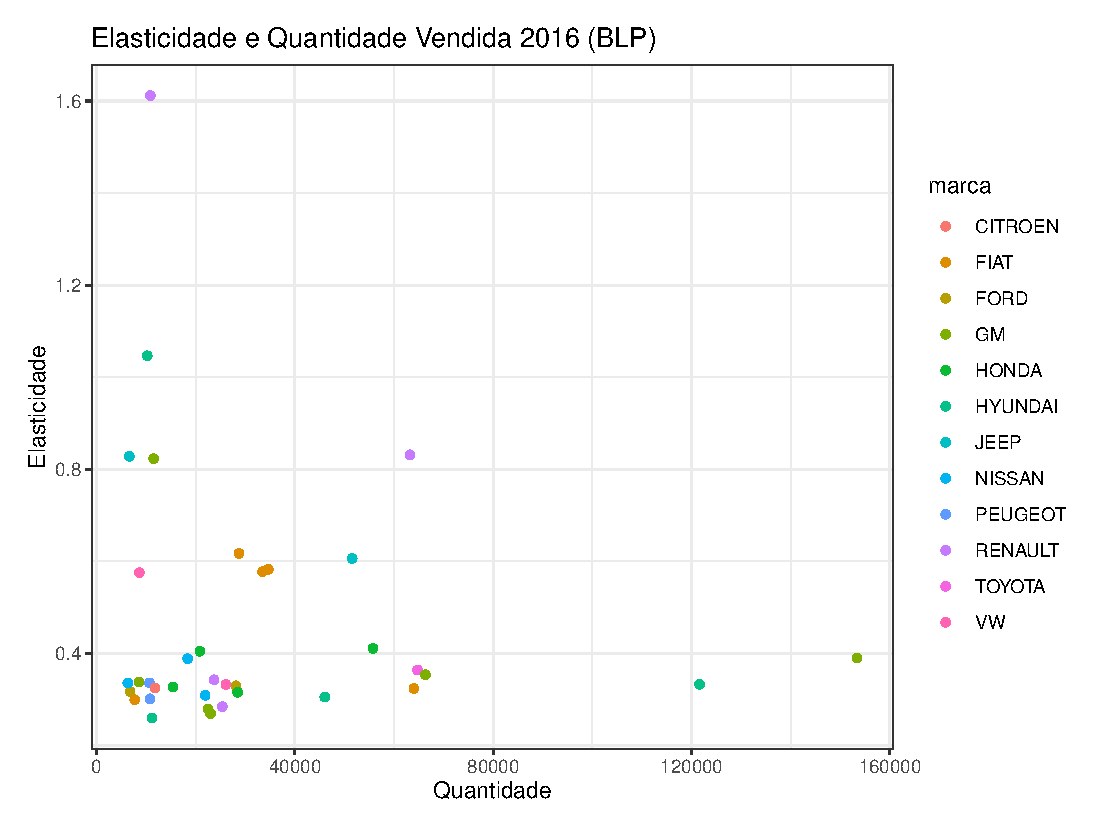
\includegraphics{figs and tabs/elasticitiesBLP.eps}
    \caption{Elasticidade e Quantidade BLP - 2016}
    \label{fig:elastblp}
\end{figure}

Pode-se perceber que não há correlação clara entre a quantidade de carros vendida de certo modelo e a elasticidade, muito diferente do resultado via Logit. Este resultado é mais realista, uma vez que espera-se que o Gol concorra mais diretamente com modelos de entrada (carros populares) de todas as marcas, que não necessariamente são os mais bem sucedidos comercialmente. A partir da metodologia utilizada na Questão 7, também podemos calcular os custos marginais e markups de cada modelo para o ano de 2016, como pode ser visto na Tabela \ref{tab:custoblp}:

\begin{table}[H]
    \centering
\begin{tabular}{r|l|l|r|r|r|r|r}
\hline
ano\_ref & marca & modelo & qtdd\_total & mkt\_sh & preco\_media & cmg\_BLP & markup\\
\hline
2016 & PEUGEOT & 2008 & 10692.000 & 0.0001591 & 74405.20 & 72214.51 & 0.0303358\\
\hline
2016 & PEUGEOT & 208 & 10768.000 & 0.0001602 & 56625.92 & 54633.13 & 0.0364760\\
\hline
2016 & CITROEN & C3 & 11824.001 & 0.0001759 & 54131.93 & 52204.77 & 0.0369155\\
\hline
2016 & HONDA & CITY & 15422.000 & 0.0002294 & 68537.75 & 66241.09 & 0.0346712\\
\hline
2016 & HONDA & CIVIC & 20857.000 & 0.0003103 & 89727.80 & 87185.73 & 0.0291569\\
\hline
2016 & GM & CLASSIC & 11530.000 & 0.0001715 & 33323.00 & 31488.10 & 0.0582728\\
\hline
2016 & RENAULT & CLIO & 10869.000 & 0.0001617 & 29702.67 & 27169.07 & 0.0932529\\
\hline
2016 & GM & COBALT & 22466.000 & 0.0003343 & 55402.88 & 53285.34 & 0.0397396\\
\hline
2016 & JEEP & COMPASS & 6599.000 & 0.0000982 & 108433.00 & 102207.21 & 0.0609135\\
\hline
2016 & TOYOTA & COROLLA & 64740.000 & 0.0009632 & 83003.17 & 80725.14 & 0.0282196\\
\hline
2016 & RENAULT & DUSTER & 25373.008 & 0.0003775 & 70001.62 & 67686.10 & 0.0342098\\
\hline
2016 & FORD & ECOSPORT & 28105.000 & 0.0004181 & 73237.09 & 71026.74 & 0.0311200\\
\hline
2016 & HONDA & FIT & 28438.998 & 0.0004231 & 63805.50 & 61577.88 & 0.0361756\\
\hline
2016 & FORD & FOCUS & 6766.000 & 0.0001007 & 80937.12 & 78643.32 & 0.0291672\\
\hline
2016 & VW & GOL & 57390.000 & 0.0008539 & 42268.40 & 40409.23 & 0.0460085\\
\hline
2016 & HYUNDAI & HB20 & 121616.001 & 0.0018094 & 50040.38 & 47743.44 & 0.0481101\\
\hline
2016 & HYUNDAI & HB20S & 46023.000 & 0.0006847 & 55314.75 & 52748.10 & 0.0486586\\
\hline
2016 & HONDA & HR-V & 55758.000 & 0.0008296 & 87544.75 & 85020.61 & 0.0296886\\
\hline
2016 & HYUNDAI & IX35 & 10226.000 & 0.0001521 & 113267.50 & 104237.42 & 0.0866299\\
\hline
2016 & VW & JETTA & 8654.002 & 0.0001288 & 83585.14 & 81209.87 & 0.0292485\\
\hline
2016 & RENAULT & LOGAN & 23706.999 & 0.0003527 & 48809.56 & 46602.91 & 0.0473500\\
\hline
2016 & NISSAN & MARCH & 18375.994 & 0.0002734 & 44870.36 & 43026.32 & 0.0428583\\
\hline
2016 & FIAT & MOBI & 28731.000 & 0.0004275 & 39023.00 & 37104.81 & 0.0516964\\
\hline
2016 & GM & ONIX & 153370.980 & 0.0022819 & 47001.71 & 44997.29 & 0.0445454\\
\hline
2016 & FIAT & PALIO & 63996.010 & 0.0009521 & 51307.85 & 49259.00 & 0.0415933\\
\hline
2016 & GM & PRISMA & 66336.998 & 0.0009870 & 51526.86 & 49456.80 & 0.0418558\\
\hline
2016 & FIAT & PUNTO & 7709.000 & 0.0001147 & 57782.55 & 55661.53 & 0.0381056\\
\hline
2016 & JEEP & RENEGADE & 51563.001 & 0.0007672 & 99382.43 & 95269.50 & 0.0431715\\
\hline
2016 & RENAULT & SANDERO & 63228.004 & 0.0009407 & 50618.43 & 47913.78 & 0.0564483\\
\hline
2016 & NISSAN & SENTRA & 6288.000 & 0.0000936 & 83199.83 & 80885.35 & 0.0286144\\
\hline
2016 & FIAT & SIENA & 33478.000 & 0.0004981 & 38661.00 & 36758.83 & 0.0517472\\
\hline
2016 & GM & SPIN & 22982.000 & 0.0003419 & 61227.88 & 59038.08 & 0.0370913\\
\hline
2016 & GM & TRACKER & 8558.000 & 0.0001273 & 79829.50 & 77488.76 & 0.0302075\\
\hline
2016 & HYUNDAI & TUCSON & 11203.000 & 0.0001667 & 69960.00 & 66437.62 & 0.0530179\\
\hline
2016 & FIAT & UNO & 34626.000 & 0.0005152 & 40471.44 & 38534.57 & 0.0502632\\
\hline
2016 & NISSAN & VERSA & 21896.996 & 0.0003258 & 54264.00 & 52270.37 & 0.0381407\\
\hline
2016 & VW & VOYAGE & 26074.004 & 0.0003879 & 50094.64 & 48135.64 & 0.0406974\\
\hline
\end{tabular}
    \caption{Custos Marginais e Markup BLP - 2016}
    \label{tab:custoblp}
\end{table}

No BLP, temos markups relativamente menores e mais homogêneos do que via Logit. A relação entre preços e markups é menos direta e linear: os modelos com maior markup são justamente o Renault Clio, o Hyundai ix35, o Renault Sandero, o Jeep Compass e GM Classic, que apresentam dispersão alta de preço. Apesar dos valores dos markups como um todo parecerem demasiadamente baixos, a relação não homogênea entre preços e markups parece mais realista do que a encontrada na Questão 7.


\bibliographystyle{ecta}
\bibliography{references}

\end{document}
